\documentclass[hyperref={colorlinks,citecolor=blue,linkcolor=blue,urlcolor=blue}, aspectratio=1610]{beamer}
\usepackage{xcolor}
\usepackage{pgfpages}
\usepackage[utf8]{inputenc}
\usepackage[english]{babel}
\usepackage{amsmath}
\usepackage{amsmath,amssymb}
\usepackage{tikz}
\usepackage{forest}


\mode<presentation>
{
  \usetheme{Madrid}       % or try default, Darmstadt, Warsaw, ...
  \usecolortheme{beaver} % or try albatross, beaver, crane, ...
  \usefonttheme{structurebold}    % or try default, structurebold, ...
  \setbeamertemplate{navigation symbols}{}
  \setbeamertemplate{caption}[numbered]
} 



\definecolor{codegreen}{rgb}{0,0.6,0}
\definecolor{codegray}{rgb}{0.5,0.5,0.5}
\definecolor{codepurple}{rgb}{0.58,0,0.82}
\definecolor{backcolour}{rgb}{0.95,0.95,0.92}

\usepackage{listings}
\lstdefinestyle{mystyle}{
    commentstyle=\color{codegreen},
    keywordstyle=\color{blue},
    stringstyle=\color{codepurple},
    basicstyle=\ttfamily\small,
    breakatwhitespace=false,
    breaklines=true,
    captionpos=b,
    keepspaces=true,
    showspaces=false,
    showstringspaces=false,
    showtabs=false,
    tabsize=2
}

% \pgfpagesuselayout{resize to}[%
%   physical paper width=8in, physical paper height=6in]

\title[IbraFSG 4: Trees and Recursion]{IbraFSG\texttrademark{} 3 - Week 8; Trees and Recursive Data Structures}


\author{Ibrahim Chehab}
\institute{UTM RGASC}
\date{\today}

\begin{document}

\begin{frame}
  \titlepage
\end{frame}

\begin{frame}{Table of Contents}
  \tableofcontents
\end{frame}

\section{Introduction}

\subsection{Welcome back to IbraFSGs\texttrademark{}}
\begin{frame}
  \frametitle{Welcome back to IbraFSGs\texttrademark{}}
  \begin{itemize}
  \item Welcome back to IbraFSGs\texttrademark{}! Hello to new people and welcome back to tenured members.
  \item This week we will be discussing \textit{Trees and Recurisve Data Structures}.
  \item Trees are a very important data structure in Computer Science, and are used in many applications. They will play a key role in the remainder of the course, and will be a main character in A2
  \item There are several types of trees:
  \begin{itemize}
    \item Binary Trees
    \item Terenary Trees
    \item Binary Search Trees (BSTs)
    \item AVL Trees [Also known as a balanced BST]
    \item Abstract Syntax Trees (ASTs) [also known as Expression Trees]
    \item Heaps
    \item Normal Trees
  \end{itemize}
  \item CSC148 Focuses on Binary Trees, BSTs, ASTs, and normal Trees
\end{itemize}
\end{frame}

\subsection{A Recap of the UltraSheet\texttrademark{}}
\begin{frame}{A Recap of the UltraSheet\texttrademark{}}
  \begin{itemize}
    \item An \textit{UltraSheet\texttrademark{}} is a "cheat sheet" that you compile for \textbf{yourself} to review course materials 
    \begin{itemize}
      \item Sharing UltraSheets\texttrademark{} is \textbf{counter-productive} and \textbf{will not help you learn the material}
      \item However, reviewing content in a group and simultaneously updating your UltraSheets\texttrademark{} is a good idea
    \end{itemize}
    \item It acts like your own personalized textbook chapter
    \begin{itemize}
      \item It allows you to \textbf{regurgitate all the course information in a contigous, organized manner} and helps you \textbf{find gaps in your knowledge}
    \end{itemize}
    \item UltraSheets\texttrademark{} help with type 1 and 2 questions 
    \begin{itemize}
      \item Can you remember what type 1 and 2 questions are?
      \item Can you remember what a \textit{type 3} question is? :troll:
    \end{itemize}
  \end{itemize}

\end{frame}

\section{Trees and Recursive Data Structures}

\subsection{Key Terms}
\begin{frame}{Key Terms}
  \textbf{Required Key Terms:} The following key terms are required for this week's content. You should be able to define and explain these terms in your UltraSheets\texttrademark{}:
  \begin{itemize}
    \item \textbf{Tree}
    \item \textbf{Parent, Child, and Ancestor}
    \item \textbf{Leaf} 
    \item \textbf{Root} 
    \item \textbf{Subtree} 
    \item \textbf{Branching Factor}
    \item \textbf{Height}
  \end{itemize}
\end{frame}

\begin{frame}{Key Terms (Cont'd)}
  \textbf{Required Key Terms:} The following key terms are required for this week's content. You should be able to define and explain these terms in your UltraSheets\texttrademark{}:
  \begin{itemize}
    \item \textbf{Tree}
    \item \textbf{Parent, Child, and Ancestor}
    \item \textbf{Leaf} \textit{Hint: These are typically your base-cases in recursive functions}
    \item \textbf{Root}
    \item \textbf{Subtree} 
    \item \textbf{Branching Factor}
    \item \textbf{Height}
  \end{itemize}
\end{frame}

\begin{frame}{Key Terms (Cont'd)}
  \textbf{Required Key Terms:} The following key terms are required for this week's content. You should be able to define and explain these terms in your UltraSheets\texttrademark{}:
  \begin{itemize}
    \item \textbf{Tree}
    \item \textbf{Parent, Child, and Ancestor}
    \item \textbf{Leaf} \textit{Hint: These are typically your base-cases in recursive functions}
    \item \textbf{Root} \textit{Hint: Think about how this can be applied recursively when writing recursive functions}
    \item \textbf{Subtree} 
    \item \textbf{Branching Factor}
    \item \textbf{Height}
  \end{itemize}
\end{frame}

\begin{frame}{Key Terms (Cont'd)}
  \textbf{Required Key Terms:} The following key terms are required for this week's content. You should be able to define and explain these terms in your UltraSheets\texttrademark{}:
  \begin{itemize}
    \item \textbf{Tree}
    \item \textbf{Parent, Child, and Ancestor}
    \item \textbf{Leaf} \textit{Hint: These are typically your base-cases in recursive functions}
    \item \textbf{Root} \textit{Hint: Think about how this can be applied recursively when writing recursive functions}
    \item \textbf{Subtree} \textit{Hint: Relate this to nested lists. Hint \#2: This term fits in very nicely with my recursion analogy from 2 weeks ago}
    \item \textbf{Branching Factor}
    \item \textbf{Height}
  \end{itemize}
\end{frame}

\begin{frame}{Key Terms (Cont'd)}
    \textbf{Reccomended Key Terms:} The following key terms are recommended for this week's content. Most are out of the scope of the course, but are fun for extra learning:

    \begin{itemize}
      \item \textbf{Graph: }A family of data structures that are used to represent relationships between objects.
      \item \textbf{Balancing Factor: }Useful in CSC263 when talking about \textit{AVL Trees} - Which are self-balancing BSTs
      \item \textbf{Cycle: }Similar to a tree, however is not strictly linearly connected.
    \end{itemize}
\end{frame}

\begin{frame}
  \frametitle{A note about today's FSG}
  \begin{enumerate}
    \item If today's FSG feels "all over the place"; that's because it is. Trees are a very broad topic, and we're only scratching the surface today.
    \item I can't go over \textit{everything} today since you're still learning about trees in CSC148
    \item Next week, we'll have more detailed and focused examples, after you've had more time to learn about trees in CSC148
  \end{enumerate}
\end{frame}

\subsection{Base Cases and Trees}

\begin{frame}[fragile]
  \frametitle{Base Cases, Recursions, and Trees}
  Recall my recursion analogy from two FSGs ago: \\
  \textit{A recursive function aims to do the least amount of work in the current recursive call before delegating the rest of the work to the next recursive call}

  How can we apply this to trees?
  
  More generally, what is the \textit{Minimum amount of work}, and what is the \textit{Work delegated}?

  \begin{center}
    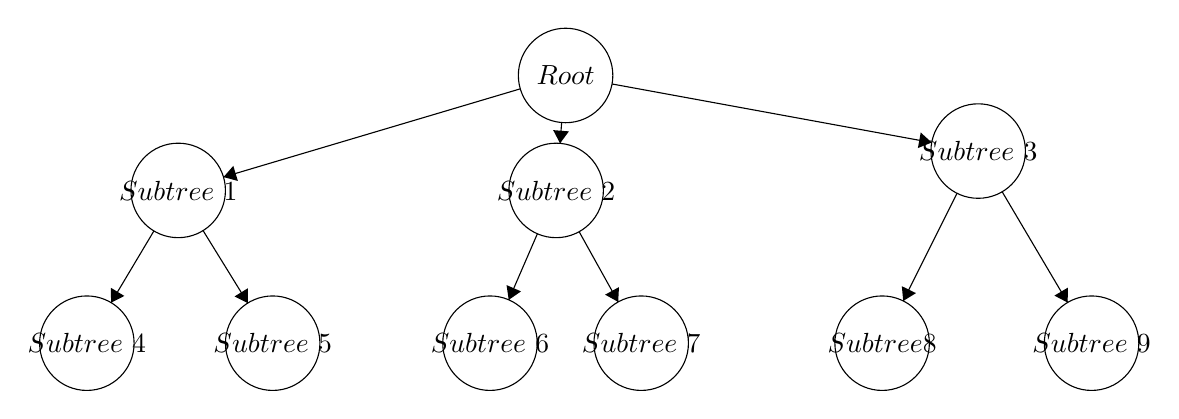
\begin{tikzpicture}[scale=0.2]
    \tikzstyle{every node}+=[inner sep=0pt]
    \draw [black] (39.5,-6.5) circle (3);
    \draw (39.5,-6.5) node {$Root$};
    \draw [black] (14.9,-13.8) circle (3);
    \draw (14.9,-13.8) node {$Subtree\mbox{ }1$};
    \draw [black] (38.9,-13.8) circle (3);
    \draw (38.9,-13.8) node {$Subtree\mbox{ }2$};
    \draw [black] (65.7,-11.3) circle (3);
    \draw (65.7,-11.3) node {$Subtree\mbox{ }3$};
    \draw [black] (9.1,-23.5) circle (3);
    \draw (9.1,-23.5) node {$Subtree\mbox{ }4$};
    \draw [black] (20.9,-23.5) circle (3);
    \draw (20.9,-23.5) node {$Subtree\mbox{ }5$};
    \draw [black] (34.7,-23.5) circle (3);
    \draw (34.7,-23.5) node {$Subtree\mbox{ }6$};
    \draw [black] (44.3,-23.5) circle (3);
    \draw (44.3,-23.5) node {$Subtree\mbox{ }7$};
    \draw [black] (59.6,-23.5) circle (3);
    \draw (59.6,-23.5) node {$Subtree\mbox{}8$};
    \draw [black] (72.9,-23.5) circle (3);
    \draw (72.9,-23.5) node {$Subtree\mbox{ }9$};
    \draw [black] (36.62,-7.35) -- (17.78,-12.95);
    \fill [black] (17.78,-12.95) -- (18.69,-13.2) -- (18.4,-12.24);
    \draw [black] (39.25,-9.49) -- (39.15,-10.81);
    \fill [black] (39.15,-10.81) -- (39.71,-10.05) -- (38.71,-9.97);
    \draw [black] (42.45,-7.04) -- (62.75,-10.76);
    \fill [black] (62.75,-10.76) -- (62.05,-10.12) -- (61.87,-11.11);
    \draw [black] (13.36,-16.37) -- (10.64,-20.93);
    \fill [black] (10.64,-20.93) -- (11.48,-20.5) -- (10.62,-19.98);
    \draw [black] (16.48,-16.35) -- (19.32,-20.95);
    \fill [black] (19.32,-20.95) -- (19.33,-20.01) -- (18.48,-20.53);
    \draw [black] (37.71,-16.55) -- (35.89,-20.75);
    \fill [black] (35.89,-20.75) -- (36.67,-20.21) -- (35.75,-19.81);
    \draw [black] (64.36,-13.98) -- (60.94,-20.82);
    \fill [black] (60.94,-20.82) -- (61.75,-20.32) -- (60.85,-19.88);
    \draw [black] (67.22,-13.88) -- (71.38,-20.92);
    \fill [black] (71.38,-20.92) -- (71.4,-19.97) -- (70.54,-20.48);
    \draw [black] (40.36,-16.42) -- (42.84,-20.88);
    \fill [black] (42.84,-20.88) -- (42.89,-19.94) -- (42.01,-20.42);
    \end{tikzpicture}
    \end{center}
    
    \textit{Hint: Think about how the term Subtree can be applied recursively, and think about the context of a subtree}

\end{frame}

\section{Practice Problems}
\subsection{Practice Problem I: TraversalOverflow}
\begin{frame}[fragile]
  
  \frametitle{Practice Problem I: TraversalOverflow}

  Dipal's computer was hit by a solar flare while he was working on his FSG Homework. As a result, all his trees were converted into their respective list representations. Unfortunately, he doesn't know what kind of traversals were used! He needs your help to match up the list representations with their respective trees.\\
  \begin{center}
    
  \begin{forest}
    for tree={circle, draw, minimum size=1em, s sep=5mm}
    [5
    [3
        [10]
        [,phantom]
    ]
    [4
      [,phantom]   
      [11]
    ]
    [8]
    [9]
]
    \end{forest}
  \end{center}
  Which of the following traversals apply to this tree? \\
  \textbf{1.} \texttt{5, 3, 10, 7, 11, 8, 9. } \textbf{2.} \texttt{5, 11, 10, 9, 8, 4, 3. } \textbf{3.} \texttt{10, 3, 11, 7, 8, 9, 5. } \textbf{4.} \texttt{10, 3, 11, 4, 8, 9, 5.}

\end{frame}

\begin{frame}[fragile]
  
  \frametitle{Practice Problem I: TraversalOverflow}
  \begin{center}
    
  \begin{forest}
    for tree={circle, draw, minimum size=2em, s sep=5mm}
    [9
    [10
        [5]
        [3]
    ]
    [8
      [7]   
      [11]
    ]
]
    \end{forest}
  \end{center}
  Which of the following traversals apply to this tree? \\
  \textbf{1.} \texttt{5, 3, 10, 7, 11, 8, 9. } \textbf{2.} \texttt{9, 10, 8, 5, 3, 7, 11} \textbf{3.} \texttt{10, 3, 11, 7, 8, 9, 5. } \textbf{4.} \texttt{10, 3, 11, 4, 8, 9, 5.}
  \textbf{Bonus!} What type of tree is this? 
  \textit{This isn't a question you can answer this week, I'm just curious who read ahead}
\end{frame}


\begin{frame}[fragile]
  
  \frametitle{Practice Problem I: TraversalOverflow}
  \begin{center}
    
  \begin{forest}
    for tree={circle, draw, minimum size=2em, s sep=5mm}
    [5
    [7
        [10]
        [3]
        [11]
    ]
    [5
      [,phantom]   
      [8
        [,phantom]
        [9]
      ]
    ]
]
    \end{forest}
  \end{center}
  Which of the following traversals apply to this tree? \\
  \textbf{1.} \texttt{5, 3, 10, 7, 11, 8, 9. } \textbf{2.} \texttt{9, 10, 8, 5, 3, 7, 11} \textbf{3.} \texttt{10, 3, 11, 7, 8, 9, 5. } \textbf{4.} \texttt{10, 3, 11, 4, 8, 9, 5.}
\end{frame}


\begin{frame}
  \frametitle{TraversalOverflow Debrief}
  What did you notice with the preoder and postorder traversals of each tree?
  \begin{enumerate}[]
    \item Were they unique?
    \item Were they bijective?
    \item Was it possible to determine the tree from the traversal, or did you need to reference the tree first?
  \end{enumerate}
  What does this tell you about the uniqueness of the pre-order and post-order traversals?
  \begin{itemize}
    \item Are they unique?
    \item Can you accurately reconstruct the tree from the traversal? Why or why not? 
    \item Is there a bijection between the traversal and the tree?
  \end{itemize}
  \textit{\textbf{Keep this in the back of your head for next week's FSG}}
\end{frame}

\subsection{Practice Problem II: To Traverse! Or Not To Traverse!}

\begin{frame}[fragile]
  \frametitle{Practice Problem II: To Traverse! Or Not To Traverse!}
  Bingleton is working on a method that will help him determine whether a given tree is a \textit{Cycle} or not.
  \textit{Note: A cycle is a tree that has a node that is both a parent and a child of itself. That is, a Node that has a child that's further up the tree.}

    \begin{lstlisting}[language=Python, style=mystyle]
class TreeNode:
  """
  Class representing a node in a tree
  """
  # Implementation omitted; Assume it's a standard TreeNode class
  
  def is_cycle(self) -> bool:
      """
      Method which determines whether the tree is a cycle or not
      """
      # TODO: Implement this method
    \end{lstlisting}

    \textit{Hint 1: Consider the type of traversal you're going to use carefully. Sometimes recursion isn't the best option.}
    \textit{Hint 2: If you choose to use recursion, consider using a helper function}

\end{frame}

\section{Conclusion}
\subsection{A Final Challenge...}

\begin{frame}
  \frametitle{A final challenge...}
As per usual, you're getting homework this week! 
\begin{center}
  \textbf{RESTRICTIONS:}
  \begin{itemize}
    \item ...None!
  \end{itemize}  
  But no, that doesn't make the question any easier :P
\end{center}

\textbf{Chicago Med's File Problem:} Dr. Choi is facing a challenging problem with organizing his medical files. His computer's hard drive contains a complex arrangement of directories and files, forming a tree-like hierarchical structure. However, he's noticed that there are numerous duplicate entries scattered throughout this structure, leading to unnecessary clutter and confusion.

To address this issue, Dr. Choi needs assistance in developing a script that will efficiently remove all duplicate file entries from his directory tree. Your task is to implement a method that takes the root node of this file system tree as input and eliminates all duplicate file entries, ensuring that each unique file is retained only once. You can assume the first entry of the file you find is the one to be kept.


\end{frame}
\begin{frame}[fragile]
  \frametitle{A final challenge\ldots}
  \begin{lstlisting}[language=Python, style=mystyle]
from __future__ import annotations

class FileNode:
    """
    Class representing a file in a file system
    
    === Representation Invariants ===
    - file_size >= 0
    len(file_name) > 0
    if default program is None, file_type is also None 
    
    """
    file_name: str
    file_size: float
    file_type: str
    default_program: str
    
    def __init__(self, file_name: str, file_size: float, file_type: str = None, default_program: str = None):
        self.file_name = file_name
        self.file_size = file_size
        self.file_type = file_type
        self.default_program = default_program
    
    def __eq__(self, __value: object) -> bool:
        return isinstance(__value, FileNode) and self.file_name == __value.file_name and self.file_size == __value.file_size and self.file_type == __value.file_type and self.default_program == __value.default_program
    
  
class FolderNode:
    """
    Class representing a folder in a file system
    """
    folder_name: str
    folder_size: float
    files: list[FileNode]
    folders: list[FolderNode]
    
    def __init__(self, folder_name: str, folder_size: float, files: list[FileNode] = [], folders: list[FolderNode] = []):
        self.folder_name = folder_name
        self.folder_size = folder_size
        self.files = files
        self.folders = folders
    
    def delete_shortcuts(self) -> None:
        """
        Method which deletes shortcuts/duplicates (Hint: Aliases) of files in the folder recursively
        """    
    \end{lstlisting}    
\end{frame}

\end{document}